\chapter{Testování}
Testování je nedílnou součástí při vývoji softwaru. Mimo ověření správné funkčnosti aplikace se také testuje, zdali bylo vytvořeno přesně to, co bylo v zadání. Rozeznáváme automatické a manuální testování. Manuální testování dělají lidé. Výběr těchto testerů by měl odpovídat cílové skupině, pro kterou je aplikace designována. Na toto testování lze nahlížet z několika aspektů. Prvním z nich je, zdali aplikace opravdu dělá to, co má a druhým aspektem je, jak~se~uživateli s aplikací pracuje. V této kapitole budou popsány různé typy testování, které byly na frameworku provedeny a testovací projekt, který byl v této souvislosti vytvořen. Software disponuje několika Unit testy, které pokrývají chování systému, které provádí složitější generování či parsování. Uživatelský test prověřil použitelnost frameworku a poskytl informace o tom, jak uživatelé pracují s aktuální verzí. Showcase projekt demonstruje možnosti a svým způsobem také testuje software. V tomto případě se jednalo o Alfa test.

\section{Unit testy}
Unit testy testují určitou část softwaru, která by měla být co nejmenší. Od toho pochází název unit, neboť se jedná o malou jednotku, jenž test pokrývá. Unit testy pokrývají většinou metody či spolupráci metod a neměli by testovat celkové chování systému. Při návrhu testů je~potřeba zvážit, zdali test přinese užitek a zdali může odhalit potencionální chybu. Například testování getterů a setterů je zbytečné. Absolutní pokrytí testů není možné z důvodů časové a prostorové náročnosti, vývoje testů, udržování a možností, které by se museli vygenerovat. Proto je vhodné testovat krajní případy a několik standardních případů použití. 

K testování byl využit framework JUnit \cite{junit}. JUnit testy se spouští při každém buildu aplikace pomocí Mavenu \cite{maven}, pokud není určeno jinak. Framework disponuje mnoha vlastnostmi, které lze použít. Integrace do existujících projektů je jednoduchá a framework podporuje anotace, pomocí kterých lze přizpůsobovat test a určovat chování testu či specifikovat výjimky, které test očekává. Testy mohou být spouštěny ve skupinách. Automatické testování pokrývají následující vlastnosti:
\begin{enumerate}
\item Test správné propagace proměnných do XML souboru s definicemi zdrojů - Do XML souborů je možné vložit hodnoty z hash mapy. Tyto hodnoty mohou za běhu ovlivňovat definici zdrojů a způsob jejich připojení. 
\item Test správné serializace dat získaných z formuláře na JSON - Z formuláře jsou získána data, která mají pouze textovou reprezentaci a na jejich základě je třeba sestavit JSON. Sestavení JSONu je potřeba ověřit.
\item Test správného vytvoření modelu na základě XML - Model je vytvářen na základě definic. Statické definice jsou součástí zdrojů a testuje se, je-li na jejich základě možné vygenerovat model. Netestují se tedy definice, ale generátor.
\item Test správného získání možností z určeného výčtového typu - V mnoha případech je~třeba získat data z výčtových typů. V tomto testu se testuje zdali algoritmus, který data získává, funguje korektně.
\end{enumerate}

\section{Uživatelský test}
Návrh frameworku zohledňoval cílovou skupinu uživatelů a snažil se přizpůsobit jejich potřebám. Při návrhu jsem čerpal ze svých vlastních zkušeností, které jsem získal při vývoji software a při své stáži v RedHatu. Firma RedHat vyvíjí v rámci jejich projektu WFK produkt RichFaces \cite{richfaces}. Jedná se o open source komponentový framework pro webové aplikace využívající technologii JSF. Tento projekt má početný tým testerů, který je napojen na~upstream. K testování se využívají JUnit testy a Arquillian testy. I přes komplexnost projektu a stabilnost frameworku, bylo rozhodnuto o jeho ukončení. Jedním z důvodů je~fakt, že~projekt dostatečně rychle nepřinesl podporu mobilních zařízení, dalším důvodem je skutečnost, že na rozdíl od svého přímého konkurenta PrimeFaces \cite{primefaces}, není tak často používaný. Tento fakt lze přikládat použitelnosti framewoku. Při použití komponent je potřeba udělat několik operací, které nemusí být pro začínající uživatele intuitivní. 

\subsection{Cílová skupina}
V mém návrhu jsem se proto soustředil na použitelnost. Cílovou skupinou jsou vývojáři, kteří chtějí knihovnu použít v nové či v stávající aplikaci. Tito vývojáři by měli mít základní zkušenost s webovými službami a v případě využití Swingové části samozřejmě s knihovnou Swing. Architekturu a způsob použití jsem se koncipoval tak, aby bylo přímočaré, nicméně bylo potřeba ověřit tuto skutečnost s uživateli během testu. Účastníky testu jsem vybíral ze~svých kolegů studentů, o nichž jsem věděl, že patří do cílové skupiny. Také jsem zvolil jako dva z testerů osoby, které již pracují jako softwarový vývojáři. Tímto výběrem jsem chtěl zajistit různorodost informací, které jsem mohl získat během testování. Test jsem provedl se~čtyřmi participanty.

\subsection{Test setup}
Vzhledem k tomu, že má framework dvě části, bylo potřeba vytvořit prostředí pro serverovou i klientskou část. Serverová část je mnohem komplikovanější, neboť vytvoření aplikace na~platformě Java~EE s restovým rozhraním a vrstvou, jež bude poskytovat data, není triviální věc a samotné nastavení serveru a tvorba tříd, které jsou zodpovědné za tuto funkcionalitu, by zabrala více času než test samotný. Takto koncipovaný test by neměl vypovídající hodnotu o využití testovaného frameworku. Testujícímu byla tedy připravena aplikace, která~již~tyto vlastnosti splňovala a obsahovala výchozí data. Uvažoval jsem o případu, kdy chce vývojář rozšířit aktuální aplikaci o tento framework. Myslím si, že toto bude v praxi nejčastější použití, neboť zatím nepředpokládáme, že by vývojáři tvořili aplikace na míru našemu frameworku. Co se týče klientské strany, byla připravena Swingová aplikace, kterou mohl participant upravovat. Klientská aplikace nedisponovala, žádnými knihovnami třetích stran. Test probíhal na mém notebooku, který měl předpřipravené prostředí. Tester mohl používat nástroj RestClient pro ověření funkčnosti serverové strany, JBDS vývojové prostředí a byla mu dodána uživatelská příručka. Před testem mu byla vysvětlena základní idea frameworku a byl mu představen framework AspectFaces, který je využit pro generování definic dat. Po~testu bylo prostředí resetováno a test se mohl opakovat.

\subsection{Test case}
Při sestavování úkolů pro testera bylo potřeba vzít v úvahu náročnost jednotlivých úkolů. Z tohoto důvodu byly koncipovány úkoly tak, aby na sebe navazovaly. Participantovi byly zadány následující úkoly v níže uvedeném pořadí.
\begin{enumerate}
\item Seznamte se se serverovou a klientskou částí. Prostudujte uživatelskou příručku.
\item Vytvořte v serverové části zdroj, který bude vracet definici dat objektu Country. Předveďte funkčnost pomocí RestClienta
\item Vytvořte v klientské části prázdný formulář, který bude sestaven na základě definice z~předchozího bodu.
\item Naplňte formulář daty ze serveru. Konkrétně zobrazte ve formuláři zemi s identifikačním číslem 1.
\item Vytvořte prázdný formulář stejný jako v bodu 3, který lze odeslat zpět na server a~po~jeho odeslání bude přidána nová země do databáze.
\item Vytvořte tabulky se všemi zeměmi v databázi a přesvědčte se, zdali byla země z předchozího bodu vložena.
\item Upravte tabulku z předchozího bodu tak, aby byla její velikost závislá na velikosti textů, které zobrazuje.
\item Vytvořte formulář z bodu 3, který bude moci upravovat zemi s identifikačním číslem 1 a po jeho odeslání se změna projeví na serveru v databázi.
\item Vytvořte formulář z bodu 3, který zobrazí zemi s identifikačním číslem 1 a po jeho odeslání bude země ze serverové databáze smazána.
\item Vytvořte formulář z bodu 3. Změňte komponentu tak, aby u proměnné active bylo místo checkboxu dropDownMenu.
\end{enumerate}
Cílem bylo zjistit, zdali jsou uživatelé schopni s frameworkem pracovat, jakým způsobem ho~využívají a jsou-li schopni pracovat s vygenerovanými komponentami. V průběhu testu jsem také vyhodnocoval jak se uživatelům pracuje s vygenerovanými komponenty. Uživatelé neměli problém při práci s těmito prvky. Tato skutečnost je způsobena tím, že jsou vygenerované formuláře standardní Swingové komponenty, na které jsou vývojáři zvyklí. Komponenty nemají také žádné skryté a nepředpokládané chování.
\subsection{Vyhodnocení}
Všichni uživatelé byli schopni splnit všechny zadané úkoly. V některých případech bylo potřeba testera trochu navést. Tyto případy zde budou rozvedeny. Po skončení testů dostali uživatelé otázku, jak se jim s frameworkem pracovalo. Participanti hodnotili práci kladně, ale~měli i pár výtek. Konkrétně měli dojem, že je framework moc chytrý. Jako příklad zde uvedu bod 3. Při plnění tohoto bodu postupovali podle uživatelské příručky, ve které jsou zobrazeny příklady definic zdrojů. Uživatelé vždy zkopírovali zdroj celý a upravili cesty ke~zdrojům. To způsobilo, že byl vygenerován formulář, který již obsahoval data. Testeři jako první zkusili vyhledat na formuláři metodu, která data odstraní, či se snažili najít metodu, která zakáže zobrazování dat. Až po nějaké době zkusili vymazat definici zdroje. Tento problém se vyskytl téměř u všech participantů. Výjimkou byl pouze jeden z nich, který nezkopíroval celou definici zdroje, ale jen jeho část. Tento participant však strávil mnohem více času definicí zdroje než jeho kolegové.

\begin{table}[width=\linewidth]
\begin{center}
\caption{Problémy se splněním jednotlivých bodů}
\label{table:userTestResult}
\begin{tabular}{|p{7cm}|p{7cm}|}
\hline
\textbf{Popis problému} & \textbf{Návrh řešení} \\
\hline
Pokud je specifikován zdroj, jsou zobrazena data ve formuláři, pokud není pak nejsou. Framework si formulář automaticky přizpůsobí. & 
Uživatelé by měli rádi větší kontrolu nad tím, jak se formulář chová. Je vhodné přidat metodu, která zapne či vypne plnění dat do formuláře. \\
\hline
Určení zdroje na základě XML. Problém byl s identifikátorem. Uživatel sice správně identifikátor zvolil, důvodem byl fakt, že ve třídě, která načítá data je identifikátor značen jako connectionKey a v konkrétních XML je reprezentován jako id. & 
Předělat název proměnné ve třídě, tak aby odpovídala XML. \\
\hline
Při vytváření tabulky chtěl uživatel provádět akce navíc. Uživatel nebyl přesvědčený o tom, zdali výměna builderu při zachování zdrojů umožní sestavit tabulku. & Je potřeba upravit uživatelskou příručku, aby tuto informaci přesně specifikovala. \\
\hline
Získání přístupu k již existující komponentě. Uživatel chvilku tápal jak získat komponentu, kterou vygeneroval. Důvodem bylo to, že uživatel chtěl komponentu získávat z panelu do kterého ji vložil. Použití správce komponent AFSwinx mu došlo až po té co si znovu přečetl uživatelskou příručku. & Možná by bylo vhodné zvážit, zdali nepřejmenovat třídu na ComponentManager či použít jiný název, který by více odrážel její funkci. Dále je potřeba upravit uživatelskou příručku a věnovat této komponentě vlastní sekci. \\
\hline
Odesílání dat na severu. Uživatel zde chvilku hledal metodu, jakou lze data odeslat. Problémem bylo to, že výsledná komponenta dědí od JPanel a nabízí tedy velké množství metod. & Řešením by bylo přidat metodu k odeslání do AFSwinx a předat jí formulář, metodu k posílání dat na komponentě je ale potřeba rozhodně zachovat. \\
\hline
\end{tabular}
\end{center}
\end{table}
Uživatelé byli s frameworkem spokojeni. Jeden z uživatelů si poté vytvořil vlastní panel, ve kterém zobrazil formulář pro vložení země do databáze, vedle něj umístil tabulku se~zeměmi a sledoval, jak se data mění. Další z nich při vytváření tabulky použil již existující kód, který mu vygeneruje formulář. Pouze změnil slovo Form na Table, prohlásil, že by to~takto mohlo fungovat a program spustil. Tabulka se mu sestavila, ale obsahovala pouze jeden prvek. Změnu zdroje, který získá všechny země, pak uživatel zvládl bez problémů. Test byl pro uživatele i časově náročný neboť se museli seznámit s frameworkem, začít ho správně používat a chybějící metody a chování doprogramovat pomocí frameworku. Během testování bylo sledováno, jak participanti ovládají vygenerované komponenty. S ovládáním komponent neměl žádný participant problém. Vygenerované formuláře a tabulky jim přišli dostatečně velké a přehledné. Při odesílání dat na server byli uživatelé schopni opravit vstupní data, pokud byla validace neúspěšná. 

\section{Ukázkový projekt}
Součástí práce je i poměrně rozsáhlý ukázkový projekt. Tento projekt je rozdělen na dvě části. Serverovou a klientskou část. Obě tyto části demonstrují použití frameworku. Serverová část je odladěna pro aplikační server GlassFish V3 a v4 \cite{glassfish}. Ukázkové projekty se využívají k tomu, aby uživateli ukázaly jak framework funguje a v některých případech i k testování, nejčastěji pokud jde vývoj knihoven. Projekt se pak používá k odladění během fáze implementace, poté k testování během fáze testování a k smoke testům před závěrečným releasem. Pokud je ukázkový projekt dostatečně rozsáhlý, zabere mnoho času rozšiřování tohoto projektu. V~našem případě bylo potřeba implementovat jak serverovou, tak klientskou část.
\subsection{Popis projektu}
Ukázkový projekt je zjednodušená aplikace sloužící k zadávání dovolených. Aplikace umožňuje žádat o dovolenou a rušit tyto žádosti. Umí spravovat uživatele, také umí vytvářet země, ve kterých se uživatel nachází, a ke kterým se váží konkrétní typy pracovní nepřítomnosti. Serverová strana využívá in-memory DerbyDB. Databázová a business vrstva je v ukázkové aplikaci spojená a manažeři, kteří jsou zodpovědní za správu dat, jsou stateless EJB \cite{javaEE}. Webové API je poskytováno pomocí knihovny RestEasy. Zabezpečení je realizováno pomocí interceptoru, který na základě basic autorizace a anotací z javax.annotation.security určí, zdali má uživatel právo k přístupu ke zdroji či nikoliv.

Klientská část aplikace využívá frameworku AFSwinx, získává data ze serverových zdrojů a ty prezentuje uživatelům. Také nabízí vytvoření formulářů a vkládání, mazání či úpravy dat. V aplikaci existuje tzv. security context, který udržuje informace o přihlášeném uživateli a v případě potřeby je odesílá na server. 

\begin{figure}[h!]
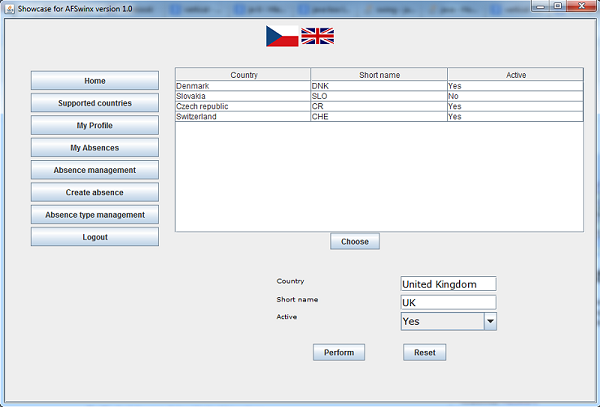
\includegraphics[width=\linewidth]{images/Country}
\caption{Ukázkový projekt - klientská část}  
\label{img:country}
\end{figure}

\subsection{Správa zemí}
Na obrázku \ref{img:country} je zobrazen náhled obrazovky, zobrazující komponenty potřebné ke správě zemí. Aby si uživatel zobrazil tyto země, je potřeba se nejprve přihlásit. Přihlášení je realizováno pomocí metody basic. Obrazovka, na které je zobrazen přihlašovací formulář, je na obrázku \ref{img:loginView}. Aplikace zobrazí všechny země, které jsou k dispozici v zadané v tabulce. Uživatel si může zemi zobrazit v detailním náhledu a popřípadě zemi upravit. Zobrazení detailních informací provede uživatel tak, že klikne na konkrétní zemi, a poté na tlačítko choose. Data jsou do formuláře propagována pomocí kontroleru bez nutnosti stahovat data ze serveru. Tato obrazovka také demonstruje možnost použití zabezpečení. V případě, že je uživatel v roli administrátora, je mu umožňěna editace těchto polí. Pokud uživatel v této roli není, pak jsou políčka needitovatelná. První vrstva zabezpečení je interpretována na straně klienta pomocí vygenerovaného uživatelského rozhraní. Druhá vrstva je na serveru. V případě obdržení požadavku na změnu se ověří, zdali má uživatel právo měnit zadaná data.
\subsection{Správa typů nepřítomností}
Každá země má svoje vlastní důvody nepřítomnosti a počet dní, které lze na tuto nepřítomnost čerpat. Na obrázku \ref{img:AbsenceType} je zobrazen náhled na správu absenčních typů. Nejprve je potřeba vybrat zemi pomocí výběrovéh menu ve vrchní části stránky. Toto menu je generovaný jednoprvkový formulář,  jehož vnitřní struktura reprezentuje identifikátor konkrétní země a uživateli je zobrazen název dané země. Po výběru konkrétní hodnoty je kontrolerem inicializována akce, při které se začne vytvářet tabulka a formulář, kterým je předán identifikátor vybrané země. Do tabulky jsou vložena data a je možné je opět měnit pomocí formuláře pod tabulkou.
\subsection{Správa nepřítomností}
Každý uživatel může žádat o schválení nepřítomnosti. Při vytváření zvolí datum začátku, datum konce a typ nepřítomnosti. Uživatel může zadat pouze typ, který odpovídá jeho zemi. Po vytvoření nepřítomnosti se mu tato nepřítomnost zobrazí v přehledu a ve správě nepřítomností ji lze měnit. Správa nepřítomností je na obrázku \ref{img:AbsenceManagementAdmin}. Upravit nepřítomnost lze pouze pokud je ve stavu Requested nebo Cancelled. V případě, že si správu zobrazí správce, může měnit nejen své nepřítomnosti, ale také nepřítomnosti ostatních uživatelů. Tuto skutečnost zachycuje obrázek \ref{img:AbsenceManagementAdmin}. Správce má k dispozici také mnohem více stavů. Data do tabulky jsou poskytována serverem na základě uživatelských rolí. Definice tabulky je pro obě role společná, nicméně definice formuláře je opět závislá na typu role. 

\subsection{Nasazení}
Aplikaci lze bez nutnosti konfigurace nasadit na aplikační server Glassfish verze 3 a 4. K~nasazení lze použít asaadmin, což je nástroj, který umožňuje ovládat aplikační server pomocí příkazové řádky. Soubor s WAR je součástí přiloženého CD či ho lze získat po spuštění mvn clean install v kořenovém adresáři. Poté je potřeba provést následující:
\begin{enumerate}
\item Rozbalte aplikační server GlassFish, který je přiložen na CD nabo si stáhnětě verzi 3 z http://www.oracle.com/technetwork/middleware/glassfish/downloads/java-archive-downloads-glassfish-419424.html Verzi 4 lze stáhnout z \\http://dlc.sun.com.edgesuite.net/glassfish/4.1/release/glassfish-4.1.zip
\item Rozbalte soubor, ve složce bin spusttě utilitu asadmin napsáním asadmin
\item Vložte následující příkaz: start-domain domain1
\item Vložte následující příkaz deploy PATHTOFILE/AFServer.war
\item Jdětě na http://localhost:8080/AFServer - zobrazí se text: I am alive. Serverová strana nedisponuje grafickým uživatelským rozhranním. Funkčnost můžete otestovat rest clienta například na adrese http://localhost:8080/AFServer/rest/country/list - content-type: application/json metoda GET.
\end{enumerate}
Klientskou část aplikace lze spustit. Spustitelný JAR soubor je na přiloženém CD či ho lze vytvořit spuštěním následujícího příkazu ve složce examples/Showaces. Příkaz je: mvn clean package assembly:single . Do složky target bude vygenerován soubor Showcase.jar, který lze spustit java –jar Showcase.jar. 
